\documentclass{article}

\usepackage{graphicx} % Graphics package
\usepackage[affil-it]{authblk} % Nice author formatting

\usepackage{float} % For figures
\usepackage{subfigure} % For subfigures
\usepackage[labelfont=bf, center]{caption} % Bolds figure titles
\renewcommand{\figurename}{Fig.} % Renames 'Figure' to 'Fig.' when called
\captionsetup{labelsep = period} % Changes : to . for captions

\usepackage{multicol} % For multi-column lists
\usepackage{verbatim} % For block commenting.

\usepackage{listings} % For code blocks.
\lstset{ % Style for code blocks.
	basicstyle=\ttfamily,
	breaklines=true,
	frame=single,
	language=Python,
	tabsize=2,
}

\usepackage{tikz} % For 2D diagrams
\usetikzlibrary{arrows,shapes,trees,shapes.geometric,positioning} % Tikz library extensions
\usepackage{rotating} % For rotate box: used here for rotating figures but keeping labels untouched


\title{UPennalizers \\Robocup 2014 Standard Platform League \\Team Description Paper}
\author{Christopher Akatsuka, Yizheng He, Jianqiao Li,\\ Tatenda Mushonga, Sagar Poudel, Junda Zhu, and\\Dr. Daniel Lee}
\affil{General Robotics Automation, Sensing and Perception (GRASP) Laboratory \\University of Pennsylvania}
\date{} %Exclude date.

\begin{document}

\maketitle

\begin{abstract}
 	This paper presents the organization and architecture of a team of soccer-playing Nao robots developed by University of Pennsylvania's Robocup SPL team. It also documents the efforts gone into improving the code base for the 2014 competitive season. All sensory and motor functions are prototyped and run in Lua on the embedded on board processors. High-level behaviors and team coordination modules are implemented by Lua using state machines. The locomotion engine allows for omni-directional motions and uses sensory feedback to compensate for external disturbances. The cognition module helps robot to detect landmarks and localize in a symmetric environment. Through the year, improvements were made across all of the various modules. 
\end{abstract}

\pagebreak
%\tableofcontents



\section{Introduction}
	In 1999, two years after the first international Robocup meet, the University of Pennsylvania formed the UPennalizers autonomous robot soccer group and began stepping up to the challenges put forth by the competition. While the league was still utilizing four-legged Sony Aibos, the UPennalizers made the quarterfinal rounds every year through 2006 before taking a brief two-year hiatus in 2007. The team reformed and returned in 2009 to begin competing in the Standard Platform League with Aldebaran Naos, taking on bipedal motion alongside improved vision techniques and advanced team behaviors. 

	Continuing its streak of making the international quarterfinals through 2012, the UPennalizers were challenged in 2013 with training a team of entirely new undergraduates without its seasoned veterans from previous years. In 2014, with existing veterans and more talents joining, the team modified the locomotion engine and rebuilt the cognition module. It went on to take first place at the 2014 US Open, and made it to the knock-out phase of Robocup 2014 in Brazil, ranking 9 of 20.



\section{Software Architecture}
	A high-level description of the software architecture for the Naos is shown in Figure \ref{fig:softarch}. The current architecture is an expansion upon the previous years work. It uses Lua as a common development platform to interface between all modules.

	The system maintains a constant update speed of 100Hz, and is decoupled into two separate pipelines. The main process handles motion control and behavior control, while an auxiliary process is dedicated solely to cognition processing. This decision allows for more efficient handling of the Nao's on-board single-core Intel Atom Z530 clocked at 1.6 GHz. The cognition engine runs off of the remaining processing power not used by the main modules, and as a result, the Naos were noted to be much more stable and robust than in previous years.

	Low-level interactions with hardware are implemented using compiled C libraries in conjunction with the Nao's on-board hardware controller (NaoQi) or custom controllers. These in turn, are called via Lua scripts, and allow for control over motor positions, motor stiffnesses, and LED's. Sensory feedback is also handled similarly, allowing users to get data from a variety of sources such as the Nao's two on-board cameras, foot weight sensors, the inertial measurement unit (IMU), and the ultrasound microphones.

	\begin{figure}[H]
		\centering
		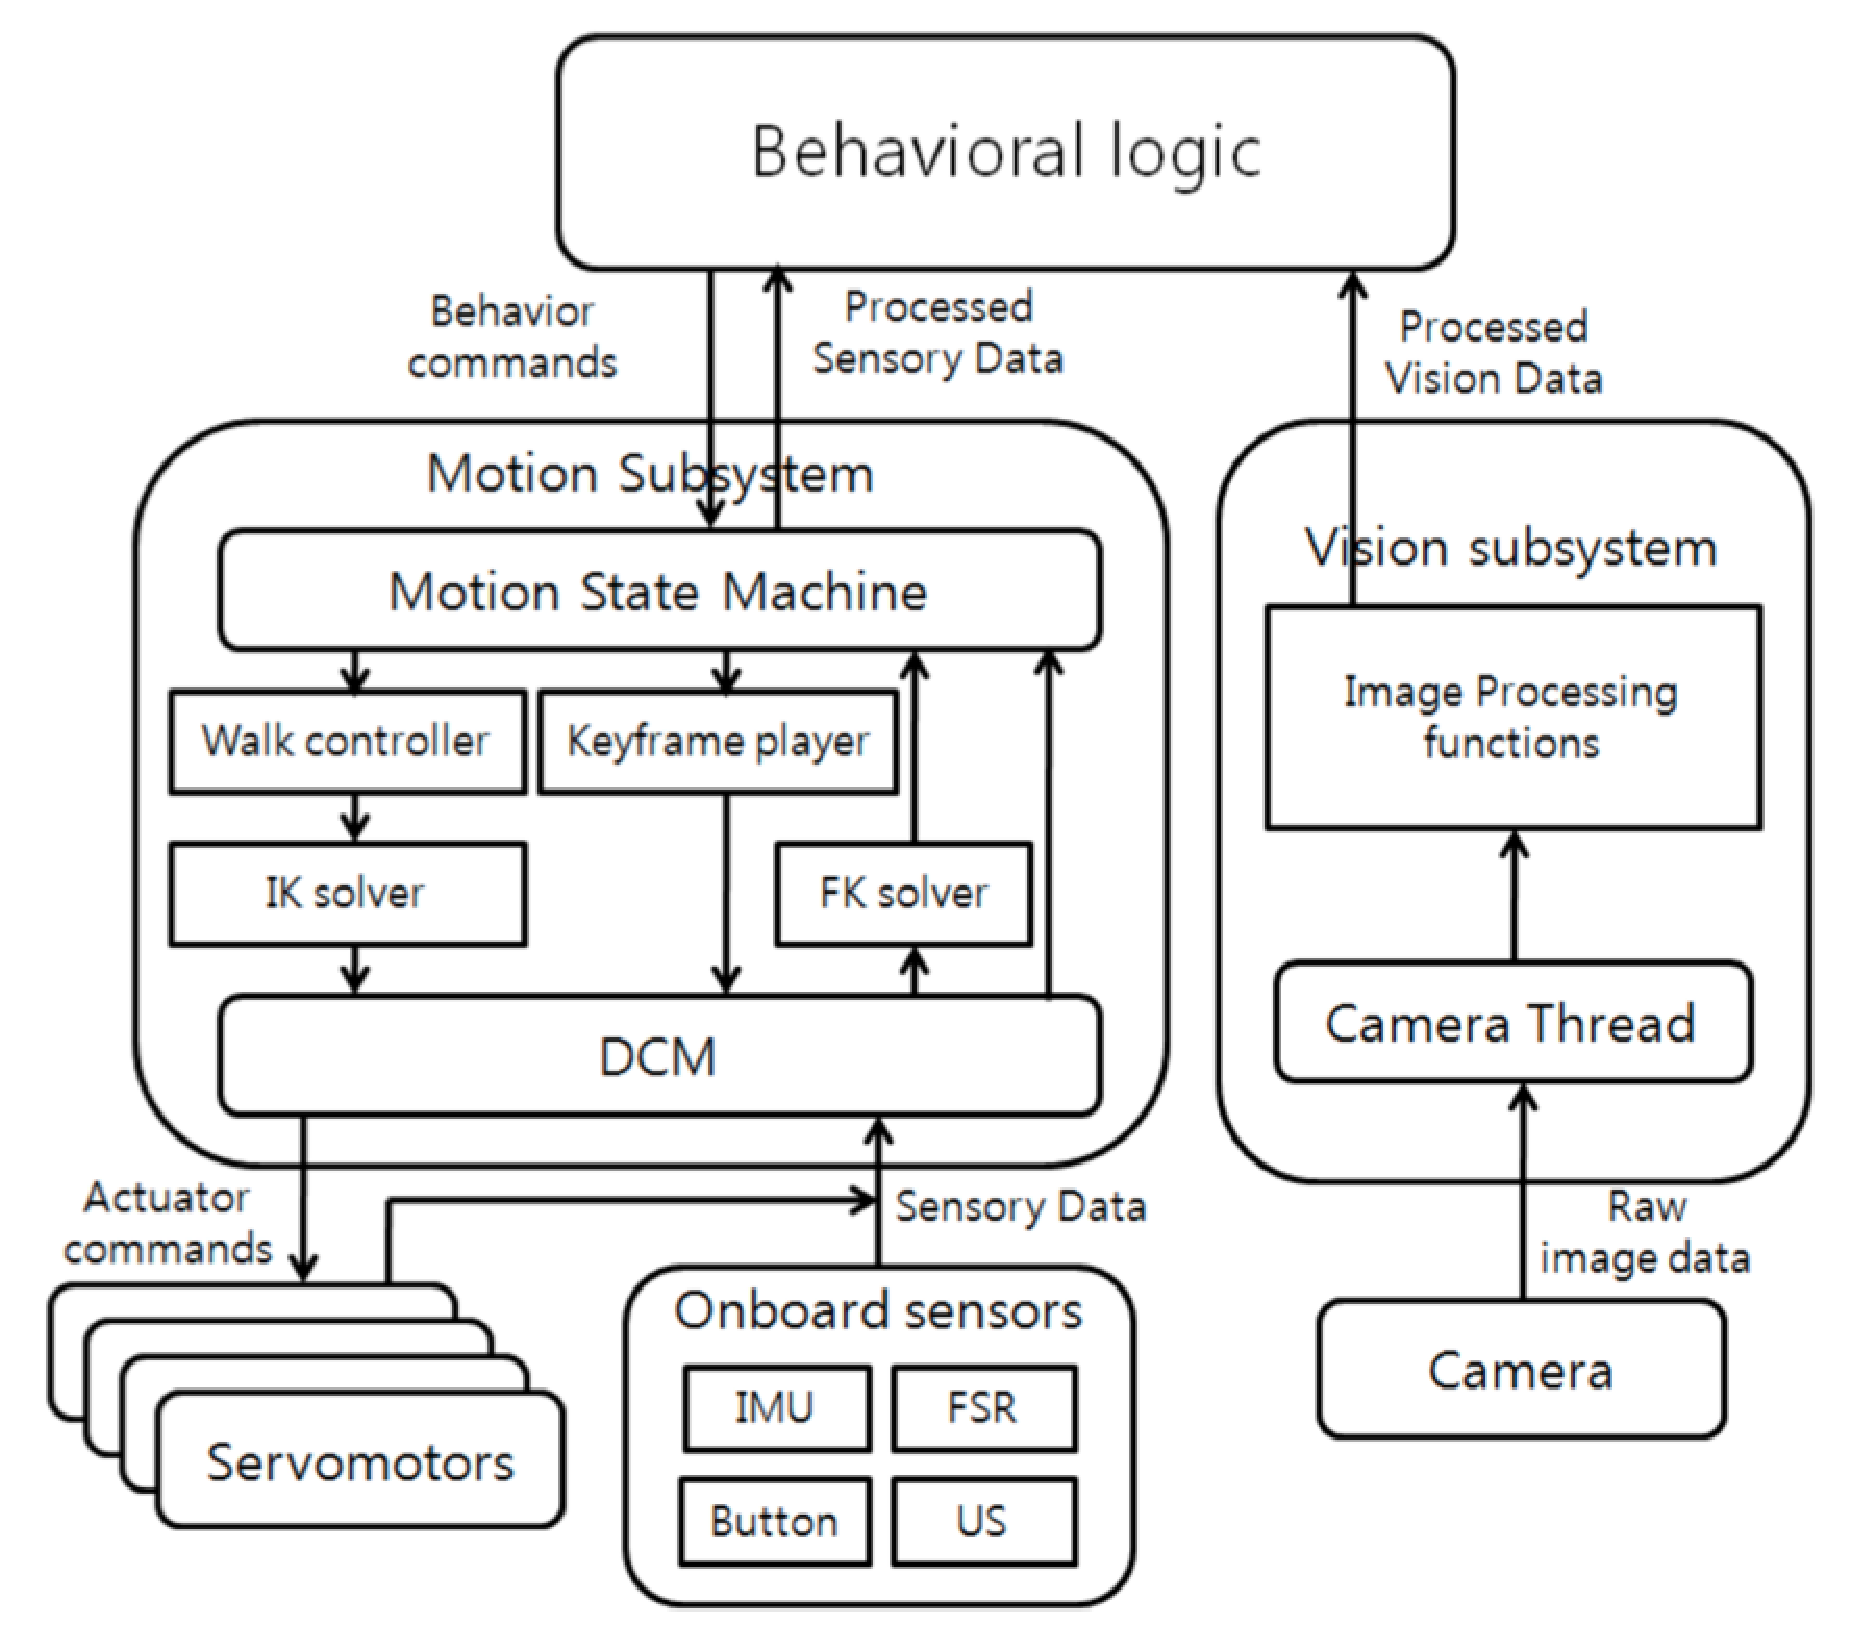
\includegraphics[width=1.0\textwidth]{figures/SoftArchOverview.eps}
		\caption{Block Diagram of the Software Architecture.}
		\label{}{fig:softarch}
	\end{figure}

	Inter-process communication is accomplished via shared memory. Important information such as ball distance, position on the field, and game state are examples of shared memory variables. Any module can write and read to shared memory. In addition, any operator connected to a Nao via secure shell can monitor the data stored in the shared memory module without any change or impact on the running system, allowing for real-time on-the-fly debugging and analysis through either Lua or MATLAB.

	The main modules accessed by our Lua routines are as follows, layered hierarchically:
	\begin{description}
		\item[Camera] Direct interface to the cameras located in the forehead (upper) and mouth (lower); controls switching frequency and bundling of images in YUYV format.
  		\item[Vision] Interprets incoming images; based on the user-created color table and camera parameters, the module passes on information relating to the presence and relatively location of key objects such as the ball, defending goal posts, attacking goal posts, field lines, field corners, and other robots.
	  	\item[World] Models the robot's state on the field, including pose and filtered ball position; 
		\item[Body] Handles physical sensory information and functions; reads joint encoders, IMU data, foot weight sensors, battery voltage, and chest button presses, but can also set motor positions, stiffnesses, and LED's.
  		\item[Motion] Dictates general movements on the Nao; i.e. sitting, standing, diving	
	  	\item[Walk] Controls omni-directional locomotion; takes in hand-tuned parameters and applies them to a zero-moment point (ZMP) based walk engine.
		\item[Kick] Maintains intra-robot stability during kick movements; different kick settings can be loaded to allow for powerful standing kicks, quick walk-kicks, and decisive side-kicks.
  		\item[Keyframes] Lists scripted positions for certain movements; getting up from front and back falls is done by feeding the Body module a series of motor positions and timings.
	  	\item[Game State Machine] Receives and relays information from the Game Controller; information from the GSM such as game state determines behavior among all robots on the field during certain times of the game.
		\item[Head State Machine] Controls head movements; different conditions determine when to switch into ball searching, ball tracking, and simply looking around.
  		\item[Body State Machine] Dispatches movement instructions; conditions from all previous modules will cause the Nao to switch between chasing after far away balls, performing curved approaches to line up for shots, dribbling, and performing kicks when the ball is close enough.
	  \end{description}



\section{Cognition}
	The cognition module acquires visual information from cameras and returns locations of key objects on the field, as well as the position of the robot itself. Figure \ref{fig:cog} shows the framework of the cognition module. 

	\begin{figure}[H]
		\centering
		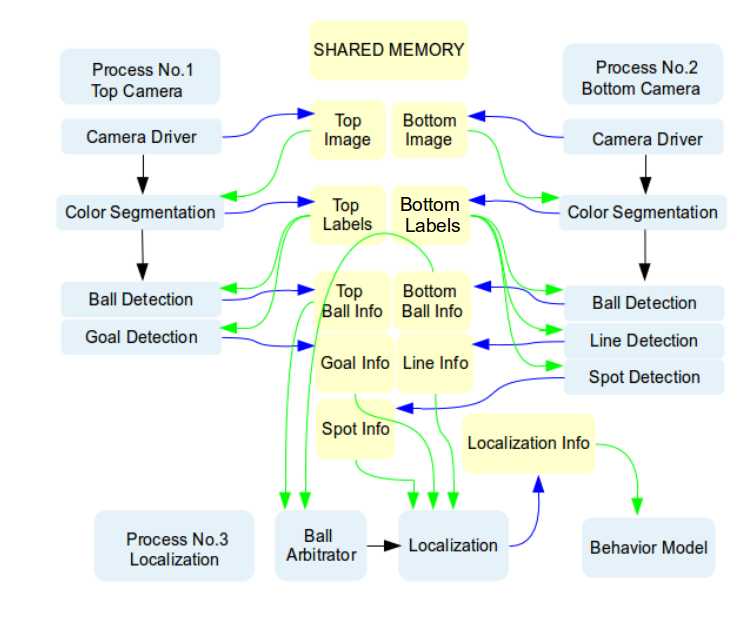
\includegraphics[width=1.0\textwidth]{figures/CogStructure.png}
		\caption{Block Diagram of the Cognition Module.}
  		\label{fig:cog}
	\end{figure}

	Each Aldebaran Nao robot has two cameras on board, also know as the top (forehead) and bottom (mouth) camera. They feed images in stream at 30 frames per second each. Images from the top and bottom cameras are processed simultaneously by two processes. Different object detection routines are run on images from different cameras to improve efficiency. An arbitrator process coordinates intermediate results from the two processes and runs the localization module. The final results from the cognition module are sent to behavior controls.

\subsection{Image Processing}
	Algorithms used for processing visual information are the same for both camera processes, and they are similar to those used by other Robocup teams. 

	The first step is color segmentation. A Gaussian mixture model is used to partition the YCbCr color cube into seven colors:

	\begin{itemize}
		\item Orange (Ball)
		\item Yellow (Goals)
		\item Green (Field)
		\item White (Lines)
		\item Pink (Robot Jerseys)
		\item Blue (Robot Jerseys)
		\item Black (Others)
	\end{itemize}

	The actual calibration process follows a supervised learning routine: images taken from both cameras are trained to form a color look-up table. While the robot is running, the image processing pipelines segment raw images into discretely colored images by classifying individual pixels based upon their mapped values in the color table. The segmented images are further shrunk to lower-resolution colored labels by merging adjacent pixels. Figure \ref{fig:unprocessed} to \ref{fig:labelb} show each step of color segmentation.

	\begin{figure}[H]
		\centering
		\subfigure[Raw Image]{
			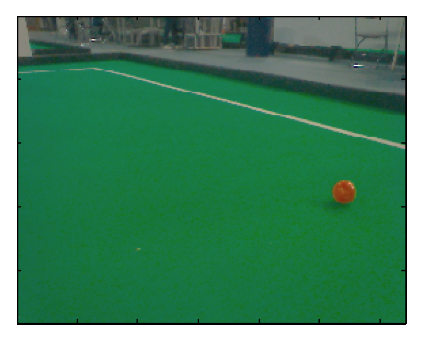
\includegraphics[width=.6\textwidth]{figures/Unprocessed.eps}
    			\label{fig:unprocessed}
		}
    		\quad
		\subfigure[Segmented Image]{
  	  		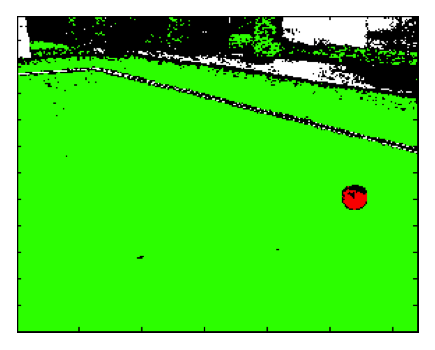
\includegraphics[width=.4\textwidth]{figures/Processed.eps}
			\label{fig:processed}
		}
    		\quad
 		\subfigure[Colored Label]{
			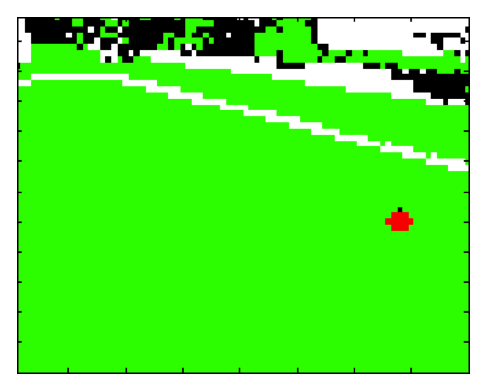
\includegraphics[width=.4\textwidth]{figures/LabelB.eps}
    			\label{fig:labelb}
		}
  	      \caption{}
	\end{figure}



	The next step is object detection on colored labels. Connected regions are recognized as either connected components or edge regions, and objects are recognized from the statistics - such as the bounding box of the region, the centroid location, and the chord lengths in the region - of the colored regions. In this manner, the location of the ball and goal posts are detected. 

	Field line recognition follows a slightly more complicate routine. Once all white pixels surrounded by green are located, a Hough transform is used to search for relevant line directions. In the Hough transform, each possible line pixel \((x, y)\) in the image is transformed into a discrete set of points \((\theta_{i},r_{i})\) which satisfy:
  
	\begin{equation}
		x \cos \theta_{i} + y \sin \theta = r_{i} 
	\end{equation}

	The pairs \((\theta_{i},r_{i})\) are accumulated in a matrix structure where lines appear as large values as shown in Figure \ref{fig:Hough}. After these lines are located, they are identified as either interior or exterior field lines based upon their position.

	\begin{figure}[H]
		\centering
		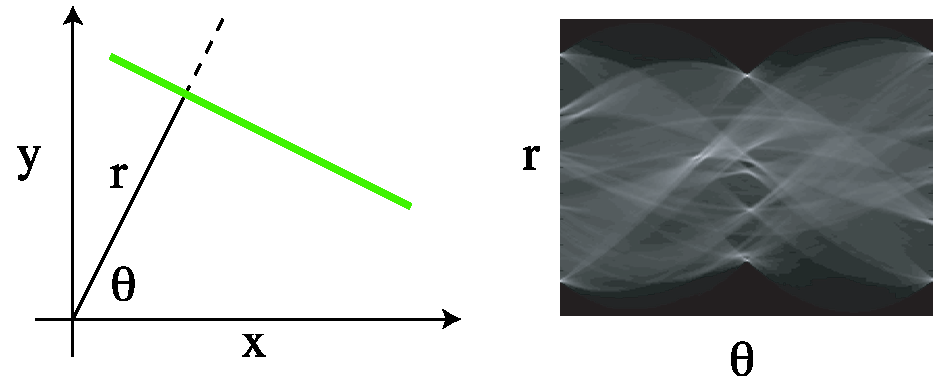
\includegraphics[width=0.8\textwidth]{figures/Hough.eps}
		\caption{Hough transformation for field line detection in images.}
  		\label{fig:Hough}
	\end{figure}

\subsection{More Details on Object Detection}


\subsubsection{Goalpost Detection}


\subsubsection{Line Detection}


\subsubsection{Ball Detection}


\subsection{Self-Localization}
	The problem of knowing the location of robots on the field is handled by a probabilistic model incorporating information from visual landmarks such as goals and lines, as well as odometry information from the effectors. Recently, probabilistic models for pose estimation such as extended Kalman filters, grid-based Markov models, and Monte Carlo particle filters have been successfully implemented. Unfortunately, complex probabilistic models can be difficult to implement in real-time due to a lack of processing power on robots. This issue is addressed with a pose estimation algorithm that incorporates a hybrid Rao-Blackwellized representation that reduces computational time, while still providing a high level of accuracy. The algorithm models the pose uncertainty as a distribution over a discrete set of heading angles and continuous translational coordinates. The distribution over poses \((x,y,\theta)\), where \((x,y)\) are the two-dimensional translational coordinates of the robot on the field, and $\theta$ is the heading angle, is first generically decomposed into the product:

	\begin{equation}
		P(x,y,\theta) = P(\theta)P(x,y|\theta) = \sum\limits_{i} P(\theta_{i})P(x,y,|\theta_{i})
	\end{equation}

 	The distribution $P(\theta)$ is modeled as a discrete set of weighted samples $\{\theta_{i}\}$, and the conditional likelihood $P(x,y|\theta)$ as simple two-dimensional Gaussian. This approach has the advantage of combining discrete Markov updates for the heading angle with Kalman filter updates for translational degrees of freedom.
	\begin{figure}[H]
		\centering
		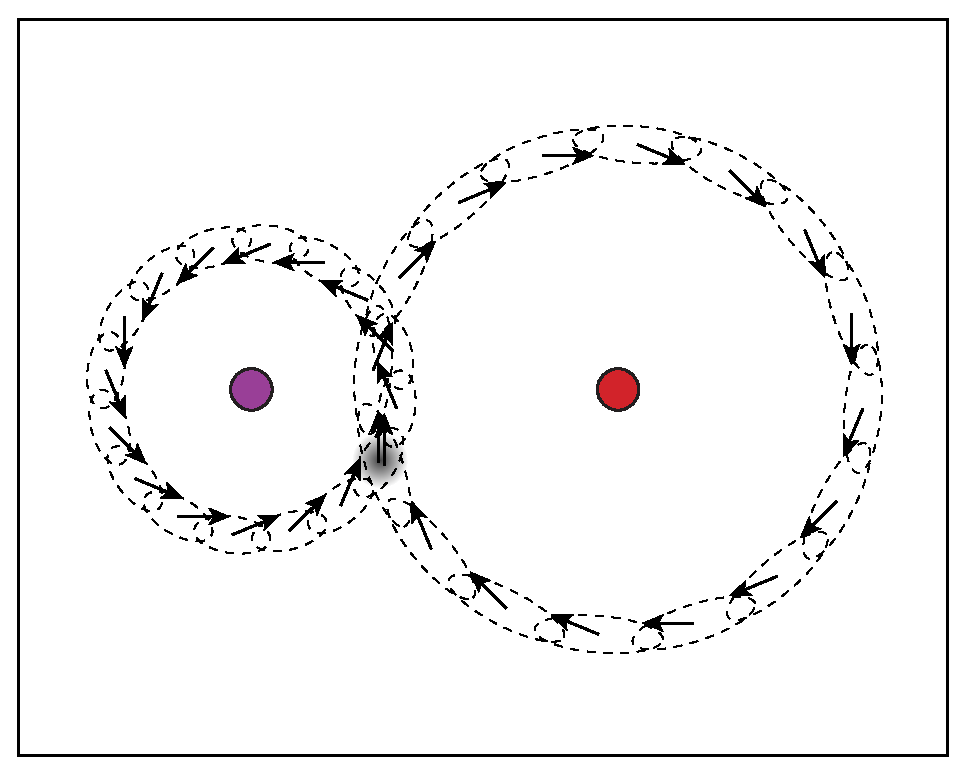
\includegraphics[width=.6\textwidth]{figures/RaoBlackwell.eps}
		\caption{Rao-Blackwellized probabilistic representation used for localization.}
		\label{fig:raoblack}
	\end{figure}
 
	This algorithm enables robots to quickly incorporate visual landmarks and motion information to consistently estimate both the heading angle and translation coordinates on the field as shown in Figure \ref{fig:raoblack}. Even after the robots are lifted ('kidnapped') by the referees, they will quickly re-localize their positions when they see new visual cues.	

\subsubsection{Particle Initialization}
	The localization algorithm utilizes 200 particles to estimate the position of the robot. Properly initializing the positions of the particles helps improve the accuracy of the localization algorithm. Before the game starts, the particles are initialized on the sides of the defending half of the field, as shown in Figure \ref{fig:Init}. In the Set state, if the robot is not manually replaced, its particles are initialized near the possible initial positions defined in our game strategy. Besides, during the game, when a robot falls down, its localization particles' heading angles are reinitialized.
    
	\begin{figure}[H]
		\centering
		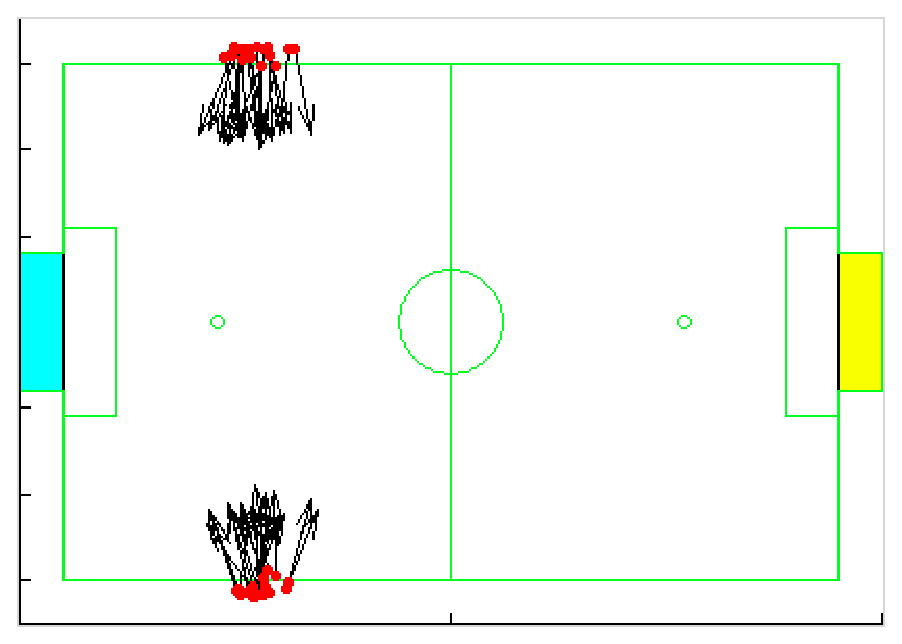
\includegraphics[width=0.6\textwidth]{figures/InitParticles}    
		\caption{Initialization of particles before game starts.}
		\label{fig:Init}
	\end{figure}

\subsubsection{Odometry, Landmark Observation and Re-sampling}
	A Kalman filter is implemented to track the continuous change on the position and weight of each particle. The filtering is a product of two steps: the motion model update and the measurement update. The motion model update - also referred to as the odometry update - utilizes the robot kinematics to update the particle filter as the robot walks around the field. Given the joint angles of the robot, forward kinematics is used to compute the location of the robot's feet as it walks. The change in translation and rotation of the body of the robot are computed based on the position of the feet, as shown in Figure \ref{fig:odometry}, and used to update the particle filter.

	\begin{figure}[H]
		\centering
		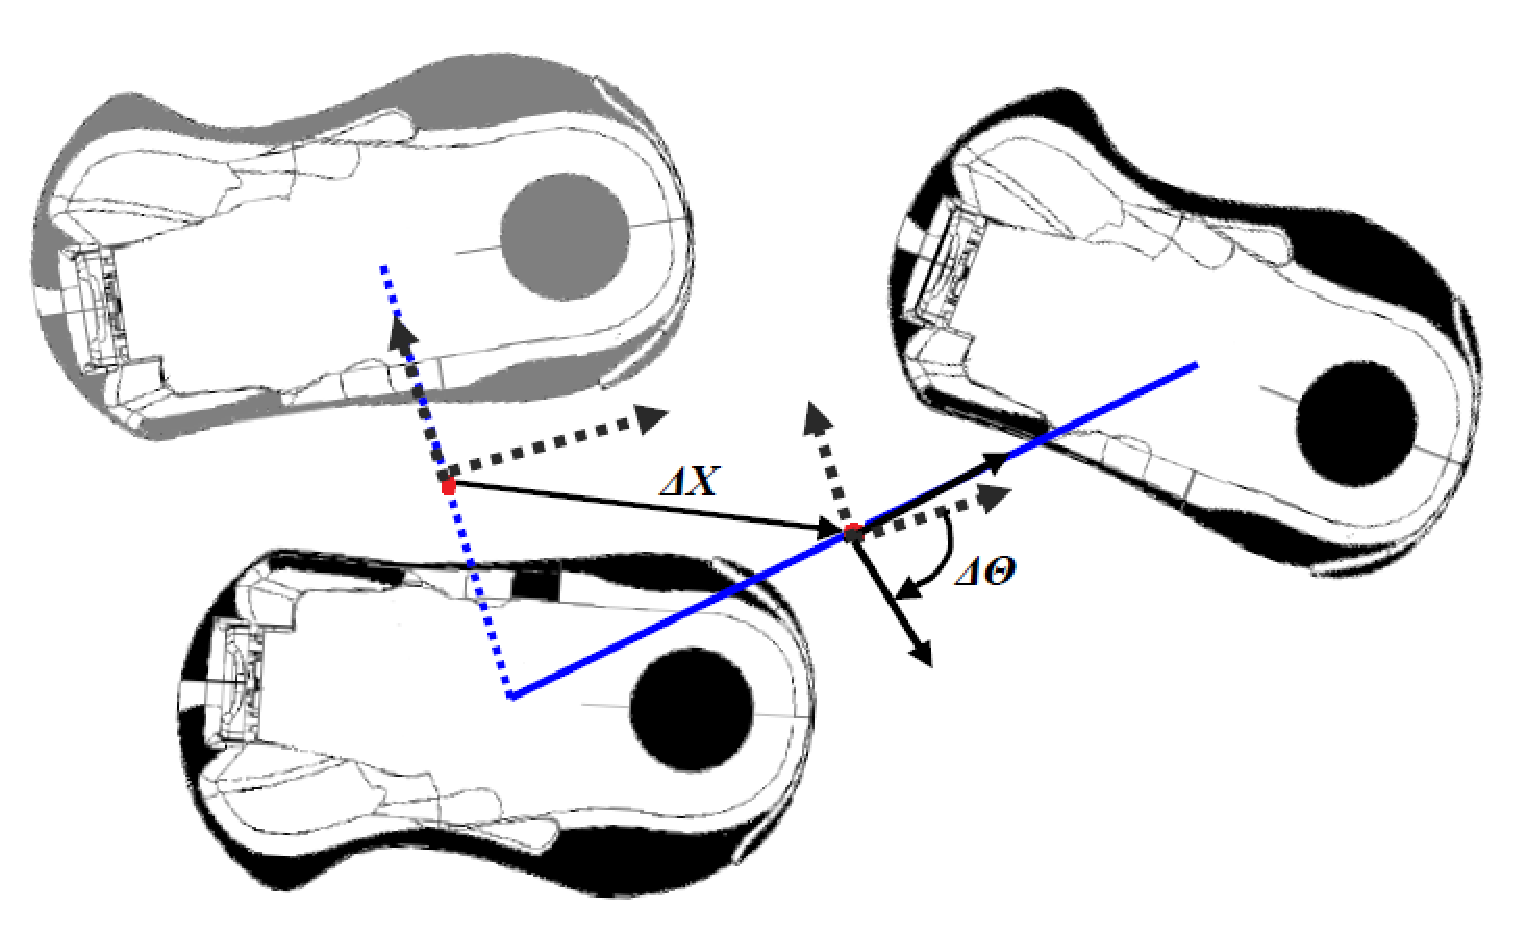
\includegraphics[width=0.6\textwidth]{figures/Odometry.eps}
		\caption{Visualization of the odometry calculation after one step.}
		\label{fig:odometry}
	\end{figure}

	The measurement model refines this estimate using sensory inputs, such as vision-based landmark detection.  The measurement model incorporates positions of landmarks to adjust the particle positions and their weights in the filter. Positions of landmarks are weighted based upon their reliability. For instance, goal post detection is considered convincing and used to correct both the position and the direction of the robot. Meanwhile, corner and line detections are only used to correct the direction due to large variance in their position calculation.

	The algorithm re-samples every 0.1 seconds. A stratification method is used to redraw all  particles so that the ones with higher weight will stay. Figure \ref{fig:particlesafter} illustrate the result of self-localization.

	\begin{figure}[H]
		\centering
		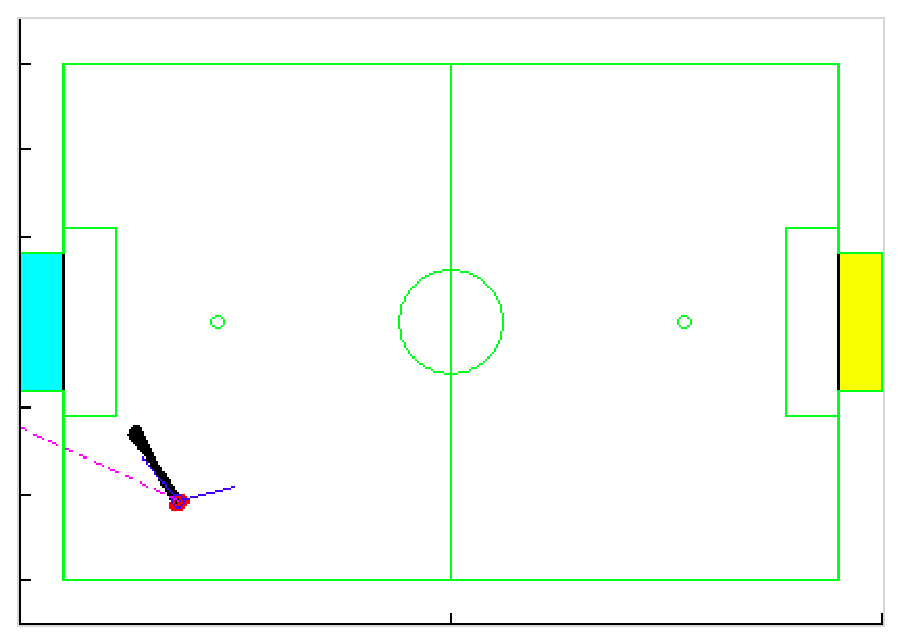
\includegraphics[width=.6\textwidth]{figures/FocusedParticles.eps}
	  	\caption{The robot weighs different landmark positions to establish an accurate estimation of its position on the field.}
		\label{fig:particlesafter}
  	\end{figure}

\subsubsection{Error Correction}
	One great challenge with self-localization in the Standard Platform League is the symmetric field. Under ideal circumstances where the robot's starting position is known, the basic particle filter approach alone is enough to keep track of the correct robot pose. However, noise in the motion model, inevitable false positive detections of landmarks, and falling down, will all eventually cause the robot to converge on a pose that is symmetrically opposite the true location. A team correcting mechanism based on goalie ball information is introduced.

	Since the goalie mostly stays in penalty box and close to the defending goal posts, it should be more confident about the location of itself and the ball than other robots on field. The correcting mechanism works when a player robot and the goalie see the ball simultaneously but believe the ball is on different sides of the field. Under such circumstances, it is very likely that the player robot's localization is flipped and its particles will be flipped back against the center of the field.

	Moreover, robots are very likely to generate localization error when they fall over near the center of the field. The correcting mechanism labels these robots as "confused players", which will not make direct shots to goal. Instead, they will dribble or slightly kick the ball until the goalie sees the ball and confirms their positions.

\begin{comment}
\subsection{Calibrating and Debugging}
    \subsubsection{Monitoring}    
      To debug the vision code, we developed a tool to receive image packets from an active robot and display them. To this end, we broadcast YUYV images,as well as two ’labeled’ images. The YUYV images represent what a robot is literally seeing at any given time, and the labeled images depict what the robot thinks it is seeing at that same time. We programmed a GUI in MATLAB which receives these packets, reconstruct them, and then displays them for the user to see. Through the use of this debugging tool, it is possible for us to test and improve our color look up tables with ease.
      \begin{figure}[H]
		    \centering
    		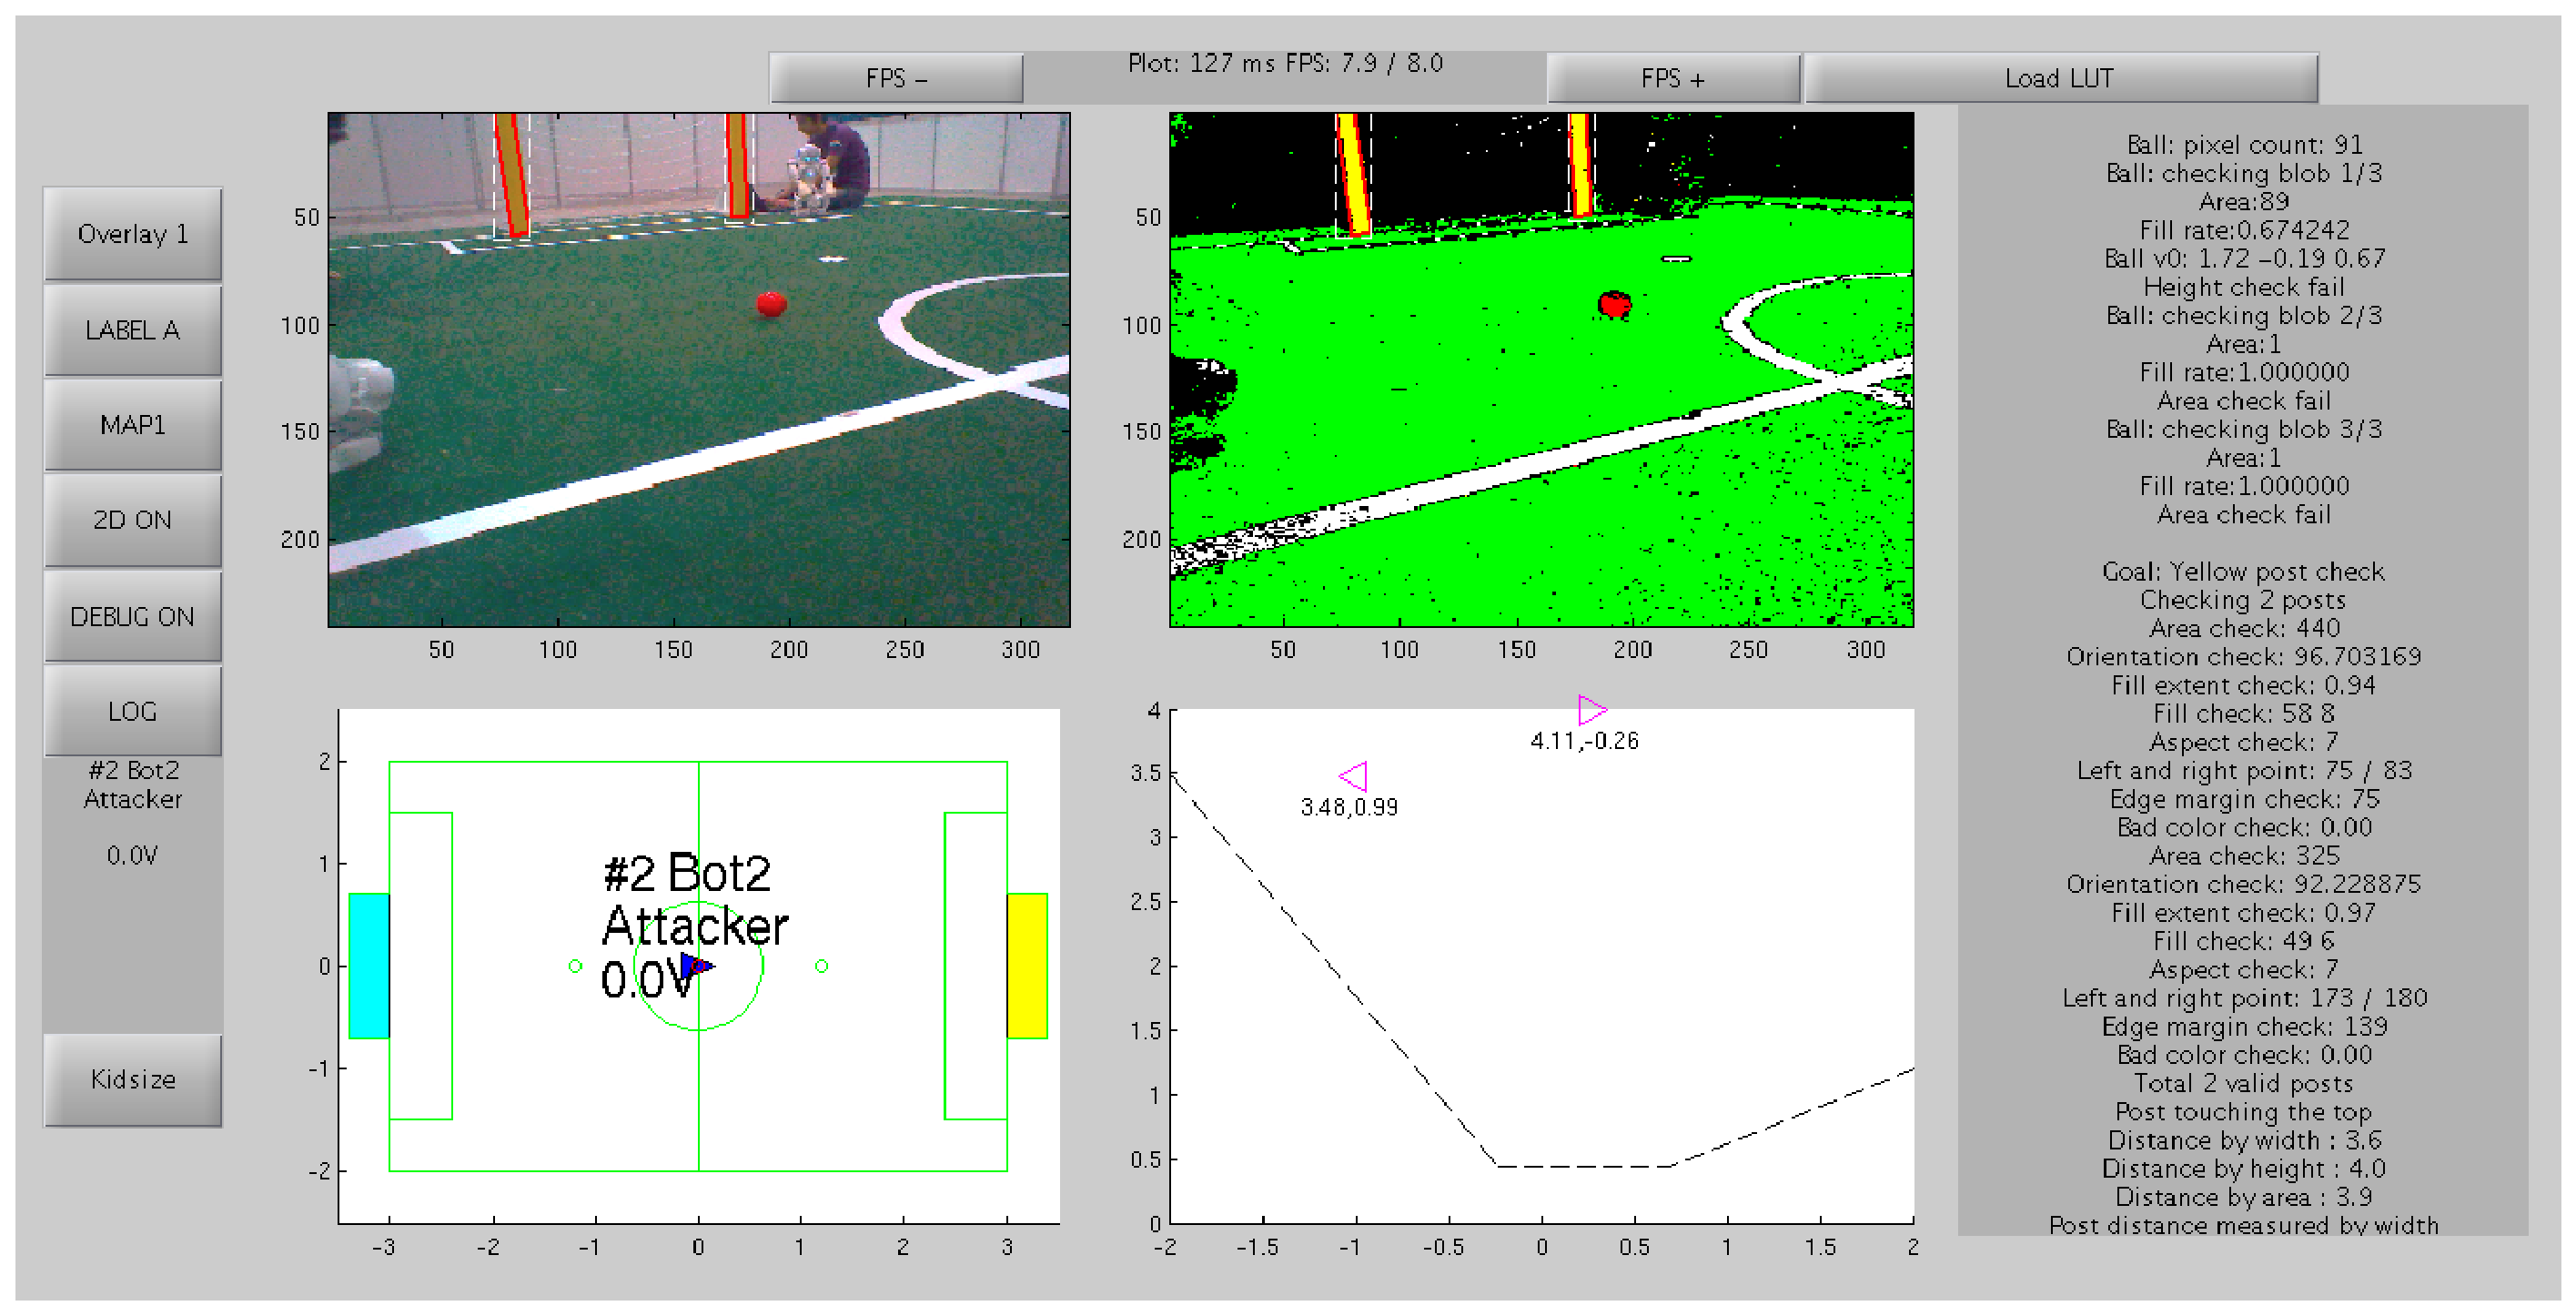
\includegraphics[width=.8\textwidth]{figures/monitor.eps}
		    \caption{Monitor for Debugging.}
    		\label{fig:monitor}
	    \end{figure}
 
    \subsubsection{Camera Parameters}
      Since vision depends highly on the quality of pictures from the camera, setting camera parameters (i.e. Exposure, Contrast, and Saturation) properly is crucial to the developing and debugging of vision code. To get better images and change parameters easily, the camera driver was modified and a Lua script was developed. Figures \ref{fig:topparams} and \ref{fig:bottomparams} display a set of camera parameter values. These parameters should make the top and bottom camera visually appear as similar as possible because both cameras’ feeds are converted using the same colortable.
 	    \begin{figure}[H]
    		\centering
		    \subfigure[Top camera]{
    			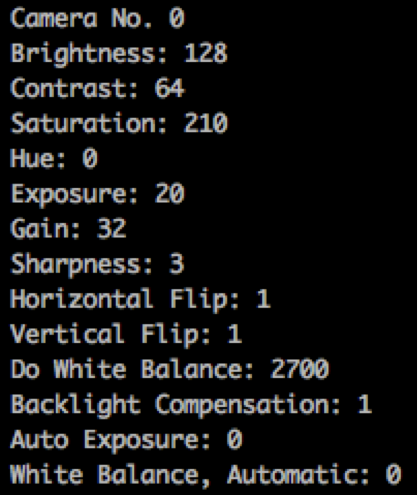
\includegraphics[width=.3\textwidth]{figures/TopCamParams.png}
		    	\label{fig:topparams}
    		}
		    \quad
    		\subfigure[Bottom camera]{
		    	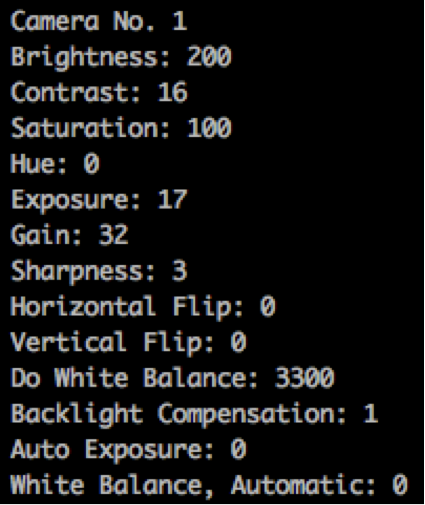
\includegraphics[width=.3\textwidth]{figures/BottomCamParams.png}
			    \label{fig:bottomparams}
    		}
		    \quad
    		\caption{Example camera parameters.}	
	    \end{figure}

	  \subsubsection{Building Colortables}
	    After camera parameters are set, pictures are taken from both cameras. Color segmentation training is then conducted through a Colortable Selection Tool, where colors of interest are associated with specific YCbCr values by a single click. Depending on the threshold value used, connected regions to the pixel clicked are also highlighted if their YCbCr values are close.
	In order to eliminate noise, we first process image packets with color definitions using a Gaussian mixture model that analyzes the probability density function of defined pixel values in conjunction with Bayes' Theorem, which expands boundaries of the color classes. As seen in the transition from Figure \ref{fig:unprocessed} to Figure \ref{fig:processed}, defined colors are displayed as a single shade in Label Mode A. Undefined colors show as black colors.
	
     	\begin{figure}[H]
		    \centering
		    \subfigure[An unprocessed image]{
			    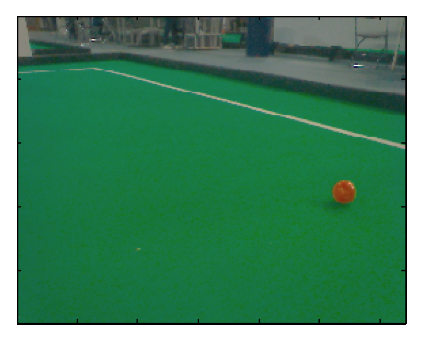
\includegraphics[width=.4\textwidth]{figures/Unprocessed.eps}
    			\label{fig:unprocessed}
		    }
    		\quad
		    \subfigure[An image in Label Mode A]{
    			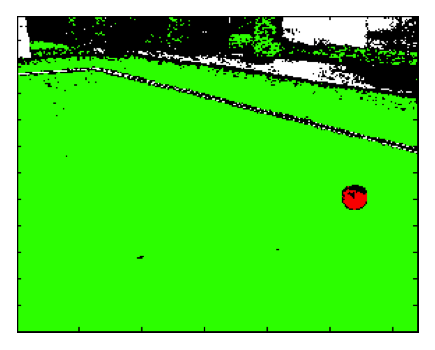
\includegraphics[width=.4\textwidth]{figures/Processed.eps}
		    	\label{fig:processed}
		    }
    		\quad
        \caption{}
    	\end{figure}

    	Next, we merge the pixels in 4x4 blocks through XOR operation assuming that target objects that are large enough that they won't be eliminated. As seen in the transition from Label Mode A to Label Mode B in Figure \ref{fig:labelb}, which is the product of these XOR's, most of the eliminated pixels were either black, undefined pixels, or noise pixels.
  
      \begin{figure}[H]
		    \centering
    		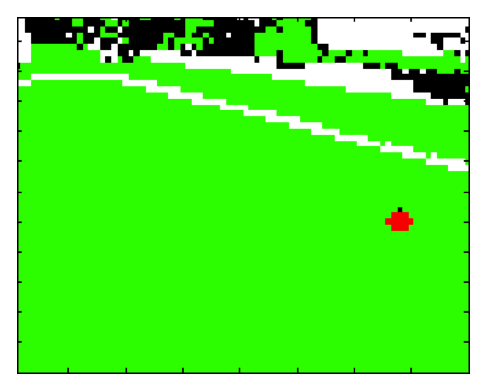
\includegraphics[width=.5\textwidth]{figures/LabelB.eps}
		    \caption{An image in Label Mode B}
    		\label{fig:labelb}
	    \end{figure}
  
    \subsubsection{Logging and Camera Simulator}
      Logging information allows the user to log vision data without affecting the currently running system in any way. These vision data are usually taken when the robot is running in a real competition environment and are thus of debugging value. We used MATLAB as our main logging program. The data we record includes:
      \begin{itemize}
        \item[--] Time Stamp
        \item[--] Joint Angles
        \item[--] IMU Data
        \item[--] YUYV Image
      \end{itemize}
  
      To better test our vision code, we developed the camera simulator in MATLAB. Instead of getting images from the robot, the simulator takes images from previous logs (generated by the logging tool) and pushes these data into the shared memory. Image processing codes can then run based on the logged images. This tool enables the user to debug the vision code without the use of a robot.
\end{comment}


\section{Motion - Jianqiao}
	Motion is controlled by a dynamic walk module combined with predetermined scripted motions. One main development has been a bipedal walk engine that allows for fast, omni-directional motions.

	The walk engine generates trajectories for the robot's center of mass (COM) based upon desired translational and rotational velocity settings. The module then computes optimal foot placement given this desired body motion. Inverse kinematics (IK) are used to generate joint trajectories so that the zero moment point (ZMP) is over the support foot during the step. This process is repeated to generate alternate support and swing phases for both legs.

	IMU feedback is used to modulate the commanded joint angles and phase of the gait cycle to provide for further stability during locomotion. In this way, minor disturbances such as carpet imperfections and bumping into obstacles do not cause the robot to fall over.

	For our 2013 season, the underlying walk engine described above was not altered; the only changes were made to parameter files dictating a few controllable variables. Depending on the surface of play, a number of these parameters need to be tuned. These include the body and step height, percentages of single- and double-support, velocity and acceleration limits, and gyroscopic feedback. These parameters are tuned by hand, and a skilled operator is able to watch a robot stumble on a new surface and know exactly what needs to be tweaked. We also opted to use a slow and stable walk that remained mostly unchanged throughout the week, opting to dedicate our efforts to behavioral and localization improvements.

	\begin{figure}[H]
		\centering
		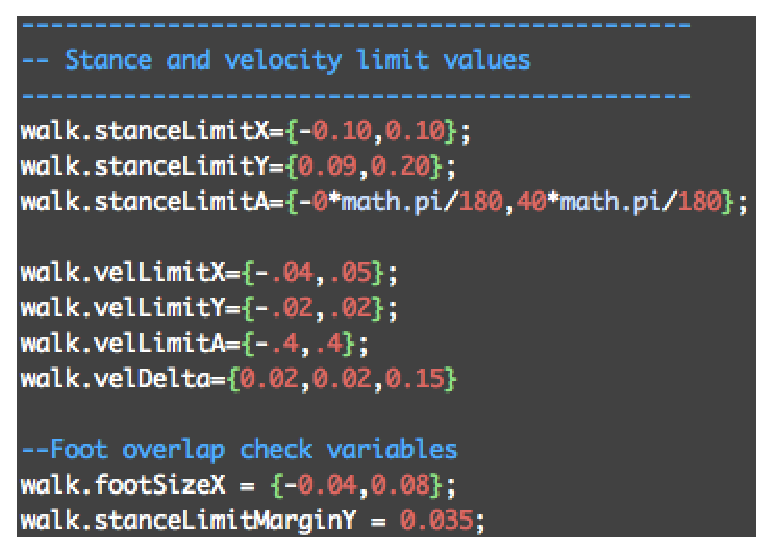
\includegraphics[width=.60\textwidth]{figures/WalkFile.eps}
		\caption{Example parameters for one of our walk files.}
	\end{figure}

  \subsection{Kicks}
	  Our kicks this year are a combination of scripted keyframes and ZMP-based kicks. Of our three kicks -- standing, walk, and side -- only the walk-kick utilizes the new ZMP engine. The old-fashioned style kicks are created by specifying motor positions and timings, and must be carefully tuned by hand in order to ensure balance, stability, and power. The new kicks are inherited from our merge with Team DARwIn. Similar to how the walk engine calculates joint positions in response to motion requests of the COM and ZMP, our newer kick calculates the way that the robot needs to balance in order to perform faster and more powerful kicks.  

	  While we utilized a mix of a keyframed standing and keyframed walk-kick during the US Open to great success, after transitioning to the ZMP walk-kick, we used this newer kick solely during our matches in Eindhoven. This allowed us to have greater control over the ball, and react quicker than opponent robots which would approach a ball and take excessive time during their keyframe motions to do a kick.

  \subsection{Keyframing}
	  A keyframe file consists of a series of frames, snapshots of the 22 motor positions along with a timing by which those positions must be reached from the previous frame. Though the motors natively read and write radians to their encoder, we use degrees and convert them later for better readability.
	  \begin{lstlisting}
  	  angles = vector.new({
	  	0.1, 25.5,
		  109.8, 11.0, -88.9, -21.4,
  		-13.7, -0.3, 17.1, -5.6, 5.2, 7.6,
	  	0.0, -1.8, 14.6, -1.1, 4.9, -2.7,
		  109.9, -10.2, 88.7, 19.9,
  	  })*math.pi/180,
	    duration = 0.400;
	  \end{lstlisting}

  	The motors in order are:
	  \begin{multicols}{3}
		  \begin{enumerate}
			  \item HeadYaw
  			\item HeadPitch
	  		\item LShoulderPitch
		  	\item LShoulderRoll
			  \item LElbowYaw
  			\item LElbowRoll
	  		\item LHipYawPitch
		  	\item LHipRoll
			  \item LHipPitch
  			\item LKneePitch
	  		\item LAnklePitch
		  	\item LAnkleRoll
			  \item RHipYawPitch
  			\item RHipRoll
	  		\item RHipPitch
		  	\item RKneePitch
			  \item RAnklePitch
  			\item RAnkleRoll
	  		\item RShoulderPitch
		  	\item RShoulderRoll
			  \item RElbowYaw
  			\item RElbowRoll
	  	\end{enumerate}
  	\end{multicols}

	  We utilize keyframed motions for two types of kicks, and also for our get-up motions. Like our walk, keyframes are hand-tuned based upon experimentation. To prolong the life of our robots, we do most of the heavy keyframe testing in Webots and then port it to the robots and perform final checks to verify full functionality.



\section{Behavior - Sagar (add goalie statemachine)}
	Finite state machines (FSMs) dictate the behaviors on our Naos and allow them to adapt to constantly changing conditions on the field. Updated at a speed of 100Hz, FSM's are analogous to flow charts. Our implementation of an FSM consists of a file that defines the transitions (\texttt{BodyFSM.lua} and \texttt{HeadFSM.lua} for the body and head, respectively) and a series of larger files that define specific states (i.e. \texttt{bodyPosition.lua} or \texttt{headSweep.lua}). A specific state consists of three main functions – entry, update, and exit. 

	As their names suggest, the entry and exit functions specify actions that need to be taken when a robot first enters a state or when it finally completes a state. An example of a typical entry action is \texttt{print(\_NAME..”entry”)}, which sends a simple print statement to the main feed and tells an operator what state a robot is currently in. Exit statements tend to be empty and are simply there to facilitate state machine functionality, but occasionally contain an action such as telling the Motion module to command a stance when leaving \textit{bodyIdle}.

	After entering and before exiting, the Nao will constantly cycle through the body of a state (the update function), querying the environment until certain conditions are met. During \textit{bodySearch}, for example, the robot will rotate in place until either a) the ball is spotted and causes a transition to \textit{bodyPosition} to determine how far away the ball is; b) it times out after a certain amount of time has been spent updating, and will transition to \textit{bodyGoToCenter} to move the robot towards the center of the field in hopes of finding a ball.

	Non-goalie behaviors are described here because they apply to a majority of the robots on the field (4 out of 5). The goalie will utilize the same transition file as a regular player, but instead uses a series of states unique only to the goalie.

	\subsection{The Body Finite State Machine (BodyFSM)}
		\begin{figure}[H]
			\centering
			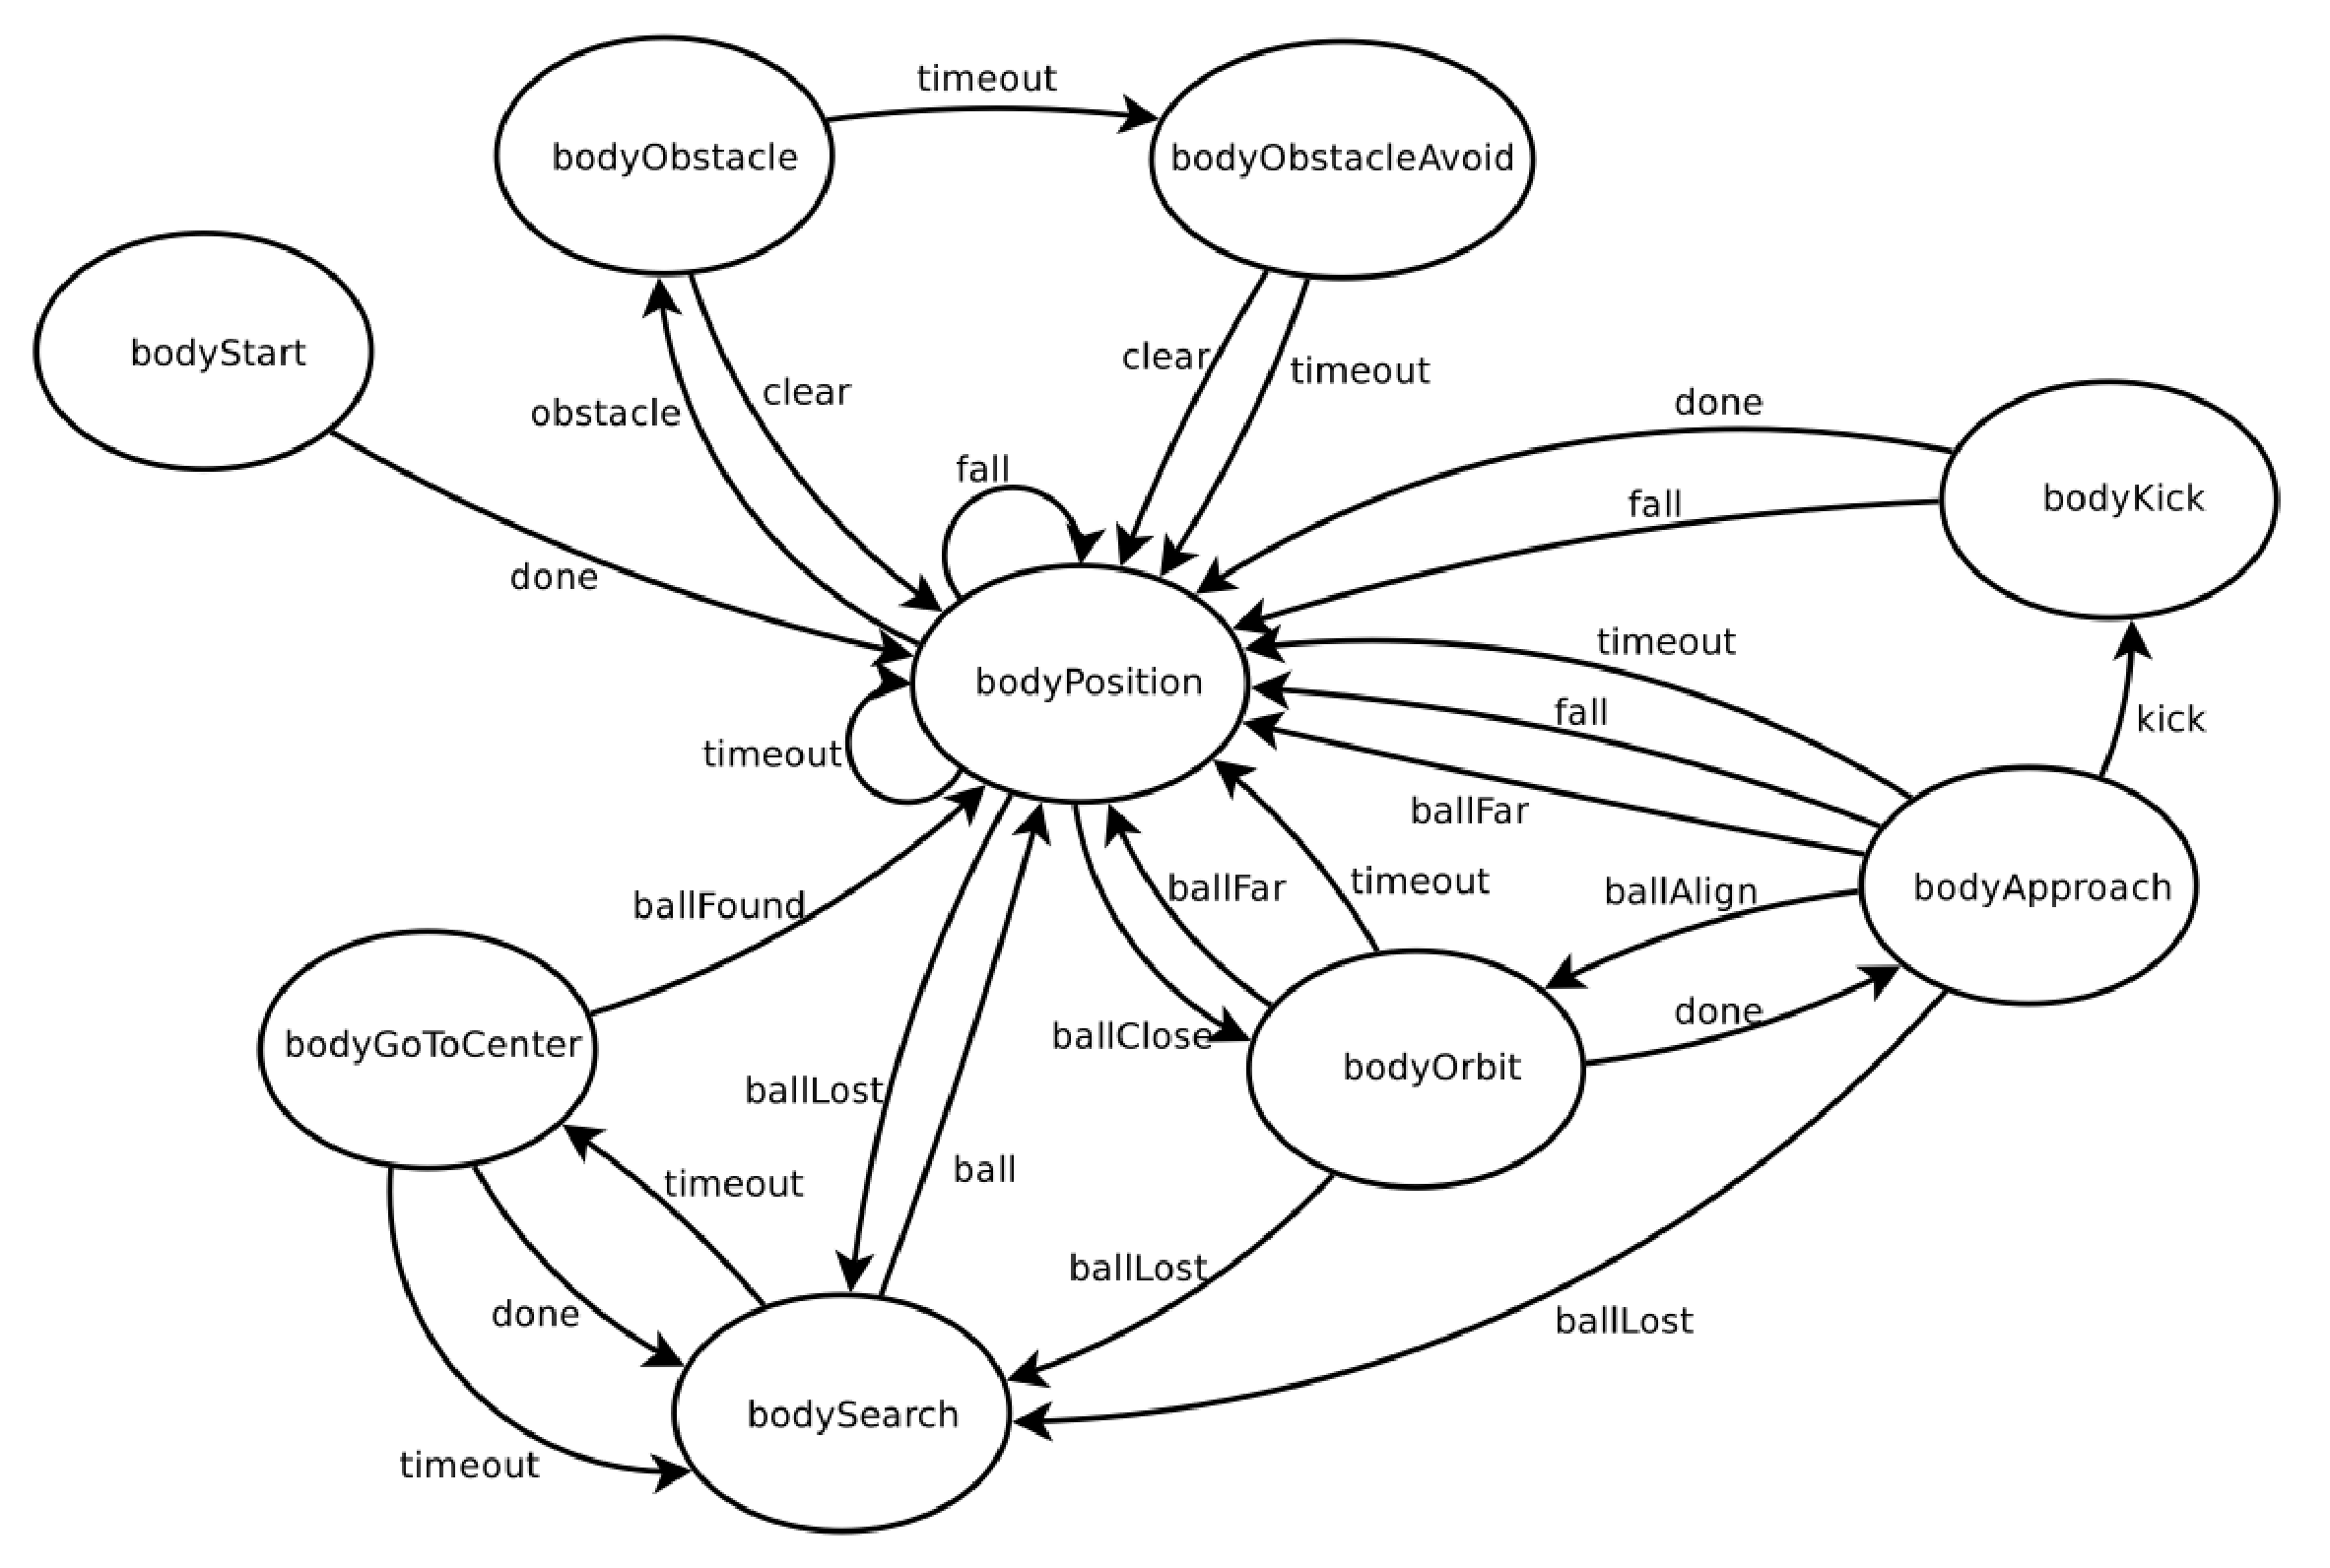
\includegraphics[width=\textwidth]{figures/BodyFSM.eps}
			\caption{Body State Machine for a non-goalie player.}
			\label{fig:bodyfsm}
		\end{figure}
		
		The specific body states used in our 2013 code are as follows:
		\begin{multicols}{2}
			\begin{description}
				\item[bodyAnticipate] Goalie specific: Prepare for the ball to come within range.
				\item[bodyApproach] Align for kick.
				\item[bodyChase] Ball sighted; run for ball and slow as distance decreases.
				\item[bodyDribble] Dribble the ball.
				\item[bodyGotoCenter] Return to the center of the field, defined as $(0,0)$.
				\item[bodyIdle] Initial state when the main code is started up. Nao will be sitting awaiting button press or game state change to 'Ready'.
				\item[bodyKick] Perform a standing kick.
				\item[bodyObstacle] Obstacle detected.
				\item[bodyObstacleAvoid] Sidestep or stop movement until the obstacle clears.
				\item[bodyOrbit] Make fine adjustments to trajectory before kicking.
				\item[bodyPosition] Main body state; most states will transition back here.
				\item[bodyPositionGoalie] Main body state for the goalie.
				\item[bodyReady] Clears temporary variables and prepares the robot to start a new half.
				\item[bodyReadyMove] After a goal has been scored or when game state is 'Ready', returns the robot to its initial position on the field.
				\item[bodySearch] Revolve and search for the ball.
				\item[bodyStart] Initial state when game goes to 'Playing'; handles kickoff.
				\item[bodyStop] Stops the robot completely.
				\item[bodyWalkKick] Perform a kick while in motion.
				\item[bodyUnpenalized] Commands the Nao to stand back up and walk into the field after being unpenalized.
			\end{description}
		\end{multicols}
		
	\subsection{The Head Finite State Machine (HeadFSM)}
		Because the head has far fewer degrees of freedom, it is much less complex than the FSM used for the body. Its overall functionality, however, remains the same as the body state machine.
		\begin{figure}[H]
			\centering
			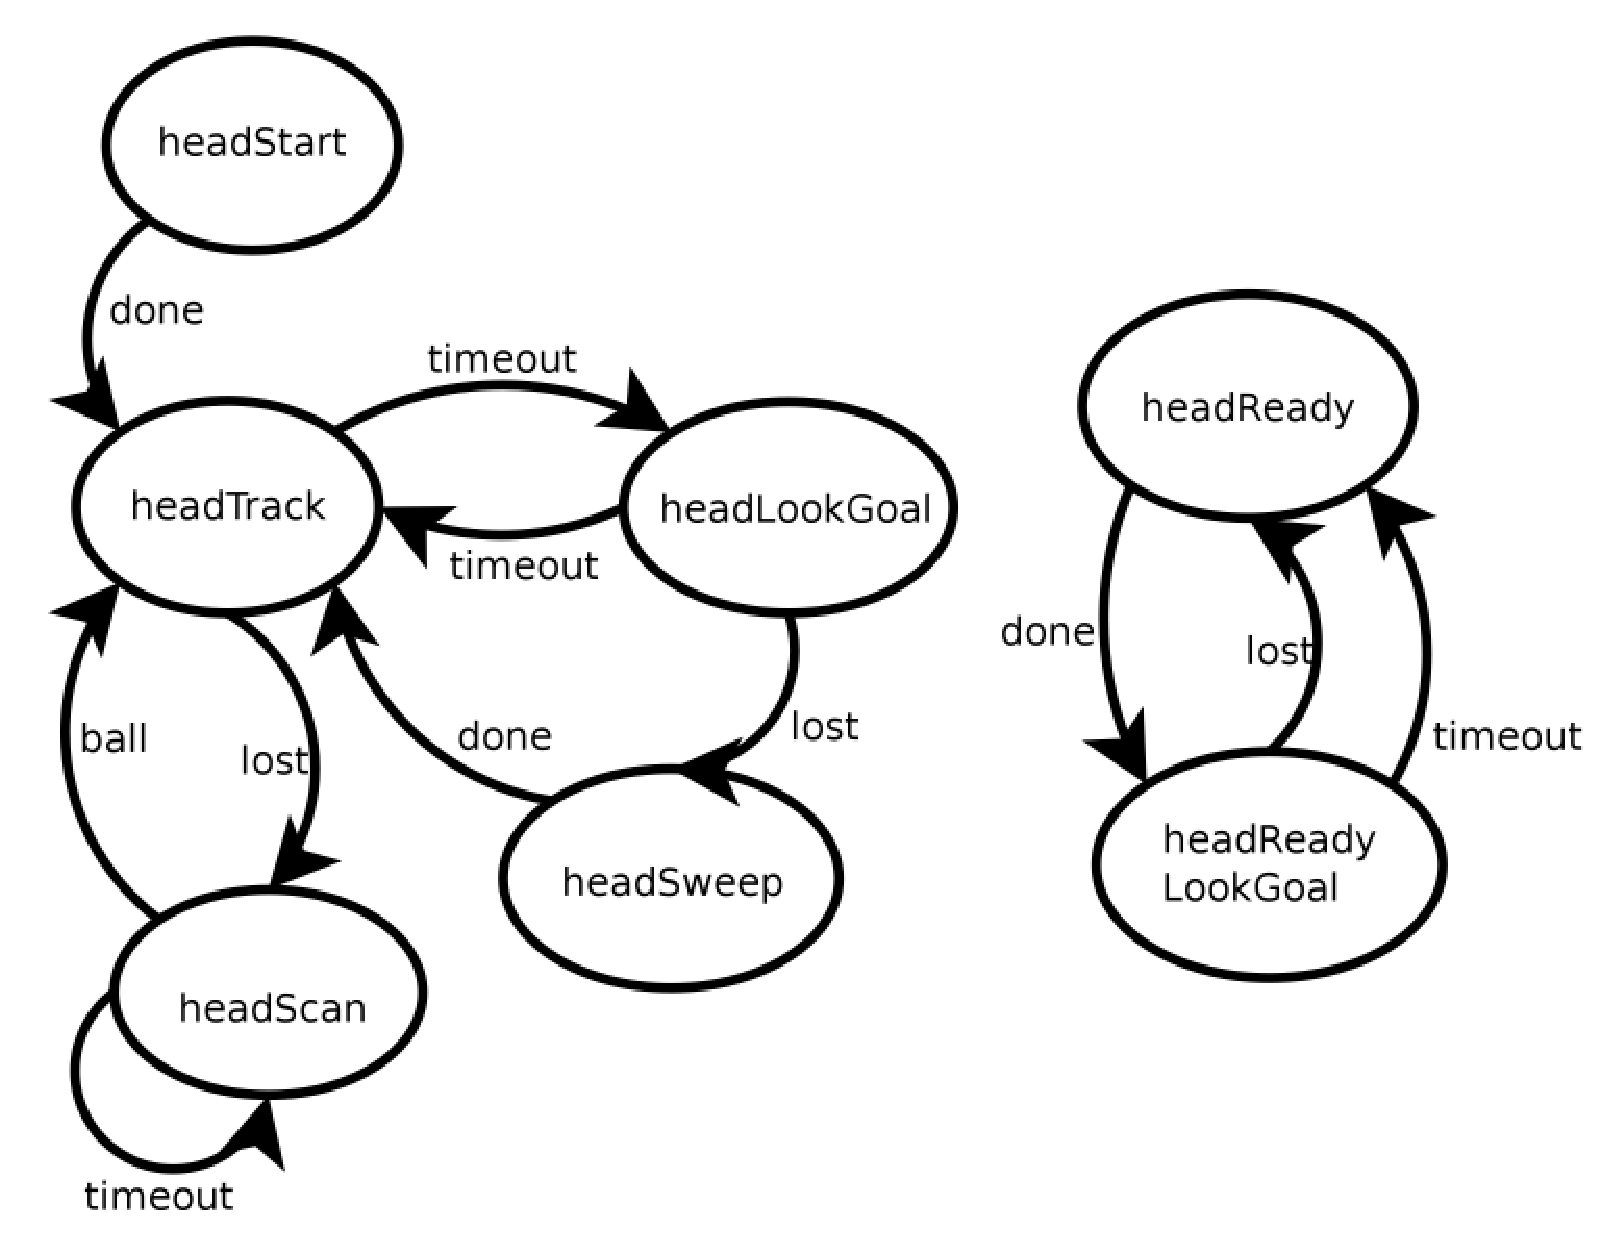
\includegraphics[width=.8\textwidth]{figures/HeadFSM.eps}
			\label{fig:headfsm}
			\caption{Head State Machine for a non-goalie player. \\Left : used while playing / Right	: Used during READY state}
			\label{fig:headfsm}
		\end{figure}

		The specific head states used in our 2013 code are as follows:
		\begin{multicols}{2}
			\begin{description}
				\item[headIdle] Initial state after main code is run; wait for game change.
				\item[headKick] During \textit{bodyApproach}, keep the head tilted down towards the ball.
				\item[headKickFollow] Follow the ball after a kick.
				\item[headLookGoal] Look up during approach to find the attacking goal posts.
				\item[headReady] Localize during \textit{BodyReadyMove} by finding lines.
				\item[headReadyLookGoal] When in the initial position, look towards the attacking goal posts to localize.
				\item[headScan] Look around for the ball.
				\item[headStart] Initial state after the game state changes to 'Playing'.
				\item[headSweep] Perform a general search, with a priority on finding goal posts.
				\item[headTrack] Track the ball, moving or stationary.
				\item[headTrackGoalie] Goalie-specific: Track the approaching ball.
			\end{description}
		\end{multicols}

  \subsection{Updates in State Machines for 2013}
    For the Body State Machine, one important improvement is the approach method. Instead of the traditional direct approach method, this year we implemented the curvature approach method, as illustrated in \ref{fig:lineapproach}, which enables the robots to quickly reach and kick the ball. We built it through careful calculation of the robot's approaching path: basically speaking, the desired position of the robot in each cycle of the state machine is changing with the attacking angle. As the robot gradually rotates to face the goal, its destination moves closer to the ball, which results in a curved path.  
 
  	Obstacle detection code was improved in preparation for this year’s competition. Data read from the ultrasound sensors allows informed decisions as to the presence of an obstacle in the robot’s path to be made. Significant filtering of the input data, as well as relative as opposed to absolute measurements, allows us to generate a relatively reliable signal. From this information, it is possible to perform avoidance maneuvers if necessary.
   
		\begin{figure}[H]
			\centering
			\subfigure[During our regular approach, the Nao approaches the ball in a straight line until getting to a certain orbit distance, and then sidesteps and rotates into position.]{
				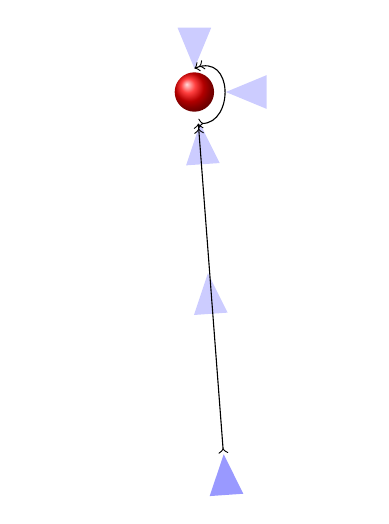
\begin{tikzpicture}
					\tikzstyle{ball} = [
						circle,
						shading=ball,
						ball color=red,
						minimum size=0.5cm
					]

					\node (ball) [style=ball] at (2.0,5.0) {};

					\node (botleft) at (0,0) {};
					\node (botright) at (4,0) {};

					\node (Nao0) at (2.4, 0) [isosceles triangle, fill=blue!40, rotate=94] {};
					\node (Nao1) at (2.2, 2.3) [isosceles triangle, fill=blue!20, rotate=94] {};
					\node (Nao2) at (2.1,4.2) [isosceles triangle, fill=blue!20, rotate=94] {};
					\node (Nao3) at (2.8,5.0) [isosceles triangle, fill=blue!20, rotate=180] {};
					\node (Nao4) at (2.0,5.7) [isosceles triangle, fill=blue!20, rotate=-90] {};
					
					\draw [>->>] (Nao0) -- (2.05,4.6);
					\draw [>->>] (2.05,4.6) .. controls (2.5,4.6) and (2.5,5.5) .. (2.0,5.3);
					
				\end{tikzpicture}

				\label{fig:linearapproach}
				}
			\quad
			\subfigure[The new curve approach that we implemented allows the Nao to perform its angle rotation during the approach, resulting in an overall faster motion to line up for kicks.]{
				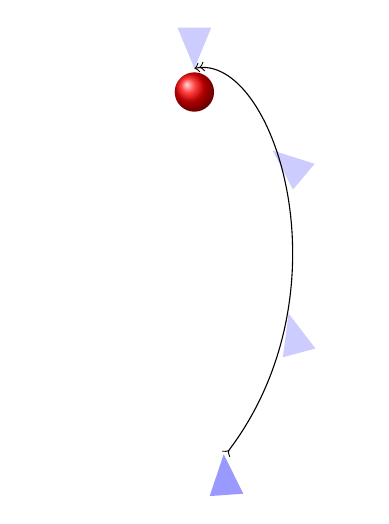
\begin{tikzpicture}

					\tikzstyle{ball} = [
						circle,
						shading=ball,
						ball color=red,
						minimum size=0.5cm
					]

					\node (ball) [style=ball] at (2.0,5.0) {};

					\node (botleft) at (0,0) {};
					\node (botright) at (4,0) {};

					\node (Nao0) at (2.4, 0) [isosceles triangle, fill=blue!40, rotate=94] {};
					\node (Nao1) at (3.3, 1.8) [isosceles triangle, fill=blue!20, rotate=105] {};
					\node (Nao2) at (3.3, 4.0) [isosceles triangle, fill=blue!20, rotate=140] {};
					\node (Nao3) at (2.0,5.7) [isosceles triangle, fill=blue!20, rotate=-90] {};
					
					\draw [>->>] (2.4,0.4) .. controls (4.0, 2.5) and (3.0, 5.5) .. (2.0,5.3);
					
				\end{tikzpicture}

				\label{fig:curveapproach}
				}
			\quad

			\caption{Difference between our original and our improved approach.}
		\end{figure}

  \subsection{Team Play}
		To make efficient use of the field, we have divided our team of five robots into 4 separate and distinct roles. These various roles have differing starting positions, and inhabit different parts of the field after kickoff. Our roles are as follows:

		\begin{center}
			\begin{tabular}{ l c p{7cm} } %p{} takes care of text wrapping by defining a fixed column width.
				Goalie & 1 & Stays in and around the defensive goal to clear the ball when it comes close. \\
				Attacker & 2 & Goes directly towards the ball and kicks. \\
				Supporter & 3 & Follows the attacking robot up-field, but stays at a respectable distance away---usually about midfield. \\
				Defender & 4 & The defending robot positions itself between the ball and defensive goal area. \\
				Defender Two & 5 & Performs double duty with the first defender, but has a different initial position. \\
			\end{tabular}
		\end{center}

		Our primary strategy is to constantly keep the ball moving down-field. To encourage this, the four general players (non-goalies) are constantly communicating over Wi-Fi, sharing their global position, relative distances to the ball, and current roles. Our code works in such a way that the role of Attacker changes often during a game, based on ETA's to the game ball. 

		\begin{figure}[H]
			\centering

			\tikzstyle{ball} = [
				circle,
				shading=ball,
				ball color=red,
				minimum size=0.5cm
			]
			
			\subfigure[The ball is closest to Nao 2, and so it is currently the Attacker. Nao 5 sights the ball, but because its distance is second farthest away, it becomes the Supporter.]{
				\begin{tikzpicture}
					\node (S) at (0, 0) [label=above:Supporter, isosceles triangle, fill=blue!30, text width=0.5cm, align=center, rotate=25] {\rotatebox{-25}{3}};
					\node (A) at +(40: 4.6) [label=left:Attacker, isosceles triangle, fill=blue!30, text width=0.5cm, align=center, rotate=-30] {\rotatebox{30}{2}};
					\node (E) at +(25: 7.0) [isosceles triangle, fill=red!30, text width=0.5cm, align=center, rotate=-150] {\rotatebox{150}{E}};

					\node (ball) [style=ball] at (4.9,2.2) {};

					\draw[->] (A) -- (ball);
					\draw[dotted, >->>] (S) -- (ball);
					\draw[dashed, o-)] (E) -- (ball);

				\end{tikzpicture}
				\label{fig:teamplay1}
				}
			\quad
			\subfigure[After the ball changes position and becomes closest to 3, it now becomes the Attacker. The Nao that was formerly an attacker, now being second furthest away, assigns itself the role of Supporter.]{
				\begin{tikzpicture}
					\node (S) at (0, 0) [label=above:Attacker, isosceles triangle, fill=blue!30, text width=0.5cm, align=center, rotate=5] {\rotatebox{-5}{3}};
					\node (A) at +(40: 4.6) [label=below:Supporter, isosceles triangle, fill=blue!30, text width=0.5cm, align=center, rotate=-118] {\rotatebox{118}{2}};
					\node (E) at +(25: 6.0) [isosceles triangle, fill=red!30, text width=0.5cm, align=center, rotate=-148] {\rotatebox{148}{E}};

					\node (ball) [style=ball] at (2.0,0.2) {};

					\draw[->] (S) -- (ball);
					\draw[dotted, >->>] (A) -- (ball);
					\draw[dashed, o-)] (E) -- (ball);

				\end{tikzpicture}

			\label{fig:teamplay2}
				}
			\quad

			\caption{Illustration of how roles change between team members.}
		\end{figure}
		
		Take for example, this situation. Following kickoff, Nao \#2, initially assigned as the Attacker, gets the ball into the opponent half. An opponent defender steals the ball away, and with a powerful kick, sends it back into our half. If Defender Two (Nao \#5) finds the ball stopped closest to him, he will inform the team that he is switching into the Attacker role. The other three general players will then check how far they are to the ball, and assign themselves roles in order of ascending distance to the ball. The next closest robot, regardless of number and initial role, would become the new Supporter, while the two furthest away would become Defenders One and Two.

    In this way, the team can reach and move the ball much quicker and with more efficiency by behaving as a dynamic unit.

	

\section{Summary}
	While the UPennalizers broke their annual tradition of making it to the quarterfinal matches every year, the team has continued to keep pace with the rest of the league. With a new batch of undergraduates ready to pass on their knowledge to new team members in the fall, the UPennalizers' future looks as bright as ever.

	Our 2013 demo code has been released on our website under the GNU public license, and we hope that it will be of use to future teams.

\end{document}

